\documentclass[12pt]{article}

% ---------------------------------
% Project Documentation (XeLaTeX)
% ---------------------------------
% Compile with: xelatex Project_Documentation.tex

\usepackage[margin=1in]{geometry}
\usepackage{setspace}
\usepackage{graphicx}
\usepackage{tabularx}
\usepackage{booktabs}
\usepackage{fontspec}
\usepackage{microtype}
\usepackage{enumitem}
\usepackage{bookmark}
\usepackage{hyperref}
\usepackage{caption}
\usepackage{array}

\setmainfont{Trebuchet MS}
\onehalfspacing

\graphicspath{{./}{./erd/}}

\hypersetup{
  colorlinks=true,
  linkcolor=black,
  urlcolor=blue,
  citecolor=black,
  pdftitle={Project Documentation: Student Study Group Finder},
  pdfauthor={UCU CSC1202 Project Team},
  pdfsubject={Web and Mobile Application Development (Project-Based Exam)},
  pdfkeywords={Study Group Finder, React, Node.js, Express, MySQL, Sequelize, JWT}
}

\setlist[itemize]{leftmargin=*, itemsep=2pt, topsep=2pt}

\begin{document}

% -------------------------
% TITLE PAGE
% -------------------------
\begin{titlepage}
\begin{center}
    
\includegraphics[width=4cm]{UCU Logo.png}\\[0.6cm]

    \textbf{\Large UGANDA CHRISTIAN UNIVERSITY}\\[0.2cm]
    \textit{A Centre of Excellence in the Heart of Africa}\\[0.8cm]

    \textbf{\large FACULTY OF ENGINEERING, DESIGN AND TECHNOLOGY}\\[0.2cm]
    \textbf{\large DEPARTMENT OF COMPUTING AND TECHNOLOGY}\\[0.2cm]
    \underline{\textbf{\large EASTER 2026 SEMESTER EXAMINATION}}\\[1.0cm]
\end{center}

\noindent
\textbf{PROGRAM:} BACHELOR OF SCIENCE IN INFORMATION TECHNOLOGY\\[0.2cm]
\textbf{YEAR:} 1 \hspace{3cm} \textbf{SEMESTER:} 2\\[0.2cm]
\textbf{COURSE CODE:} CSC1202\\[0.2cm]
\textbf{COURSE NAME:} WEB AND MOBILE APPLICATION DEVELOPMENT\\[0.2cm]
\textbf{EXAMINATION TYPE:} 100\% PROJECT-BASED EXAM\\[0.2cm]
\textbf{PROJECT DURATION:} APRIL 2026\\[1.2cm]

\begin{center}
    \underline{\textbf{\Large PROJECT DOCUMENTATION}}\\[0.2cm]
    \textbf{\Large STUDENT STUDY GROUP FINDER}\\[1.0cm]
\end{center}

\vfill
\begin{center}
    \textbf{Submission Date:} April 2026
\end{center}
\end{titlepage}

% -------------------------
% TEAM MEMBERS
% -------------------------
\section*{Project Team Members}
\addcontentsline{toc}{section}{Project Team Members}

\noindent
This project was jointly developed and submitted by the following collaborative team:

\vspace{0.4cm}

\noindent
\begin{tabularx}{\textwidth}{|c|X|l|l|}
\hline
\textbf{S/N} & \textbf{Member Name} & \textbf{Registration No.} & \textbf{Access No.} \\ \hline
1 & Nsubuga Edrine & S25B13/057 & B34863 \\ \hline
2 & Kyebambe Timothy & S25B13/128 & B36004 \\ \hline
3 & Mwebaza Sheebah & S25B13/017 & B34607 \\ \hline
4 & Nalukenge Anita & S25B13/088 & B35117 \\ \hline
5 & Namuddu Vivian Lukwago & S25B13/019 & B34609 \\ \hline
\end{tabularx}

\newpage

% -------------------------
% TABLE OF CONTENTS
% -------------------------
\tableofcontents
\newpage
\listoffigures
\newpage

% -------------------------
% 1. INTRODUCTION
% -------------------------
\section{Introduction}
\subsection{Project Overview}
The \textbf{Student Study Group Finder} is a web-based platform that supports academic collaboration by enabling students to register, discover or create study groups, join groups of interest, schedule study sessions, and communicate through posts and chat. The system is designed as a modern client--server application with a secured REST API and a relational database backend.

\subsection{Problem Statement}
Students often struggle to identify peers studying the same courses, coordinate meeting locations/times, and maintain structured group communication. Informal channels (e.g., personal messaging) can be fragmented, unmoderated, and hard to scale across multiple courses.

\subsection{Objectives}
\begin{itemize}
  \item Provide secure registration and login for students and administrators.
  \item Enable creation, discovery, and joining of study groups with clear metadata (course, faculty, location, capacity, virtual/physical).
  \item Support scheduling of study sessions within groups.
  \item Provide in-group communication via posts and chat.
  \item Maintain data integrity and role-based access control.
\end{itemize}

\subsection{Scope}
This project covers core collaboration workflows: authentication, study group management, session scheduling, and communication. It does not aim to replace official university systems (e.g., LMS), but to complement them as a student-focused collaboration tool.

% -------------------------
% 2. TECHNOLOGY STACK
% -------------------------
\section{Technology Stack}
\begin{itemize}
  \item \textbf{Frontend}: React.js (Vite), React Router, Axios
  \item \textbf{Backend}: Node.js, Express.js
  \item \textbf{Database}: MySQL
  \item \textbf{ORM}: Sequelize
  \item \textbf{Authentication}: JSON Web Tokens (JWT)
  \item \textbf{Documentation / Testing}: Postman collection (backend), Markdown/LaTeX documentation
\end{itemize}

% -------------------------
% 3. SYSTEM ARCHITECTURE
% -------------------------
\section{System Architecture}
The system follows a three-tier architecture that separates responsibilities for maintainability and scalability.

\subsection{Architecture Description}
\begin{itemize}
  \item \textbf{Client Tier (Frontend)}: A Single Page Application that renders the user interface, handles navigation, and communicates with the API using HTTP requests.
  \item \textbf{Application Tier (Backend)}: A RESTful Express API responsible for authentication, authorization, business rules, and data access through Sequelize.
  \item \textbf{Data Tier (Database)}: A MySQL relational database that stores users, groups, memberships, posts, sessions, and chat messages.
\end{itemize}

\begin{figure}[h!]
  \centering
  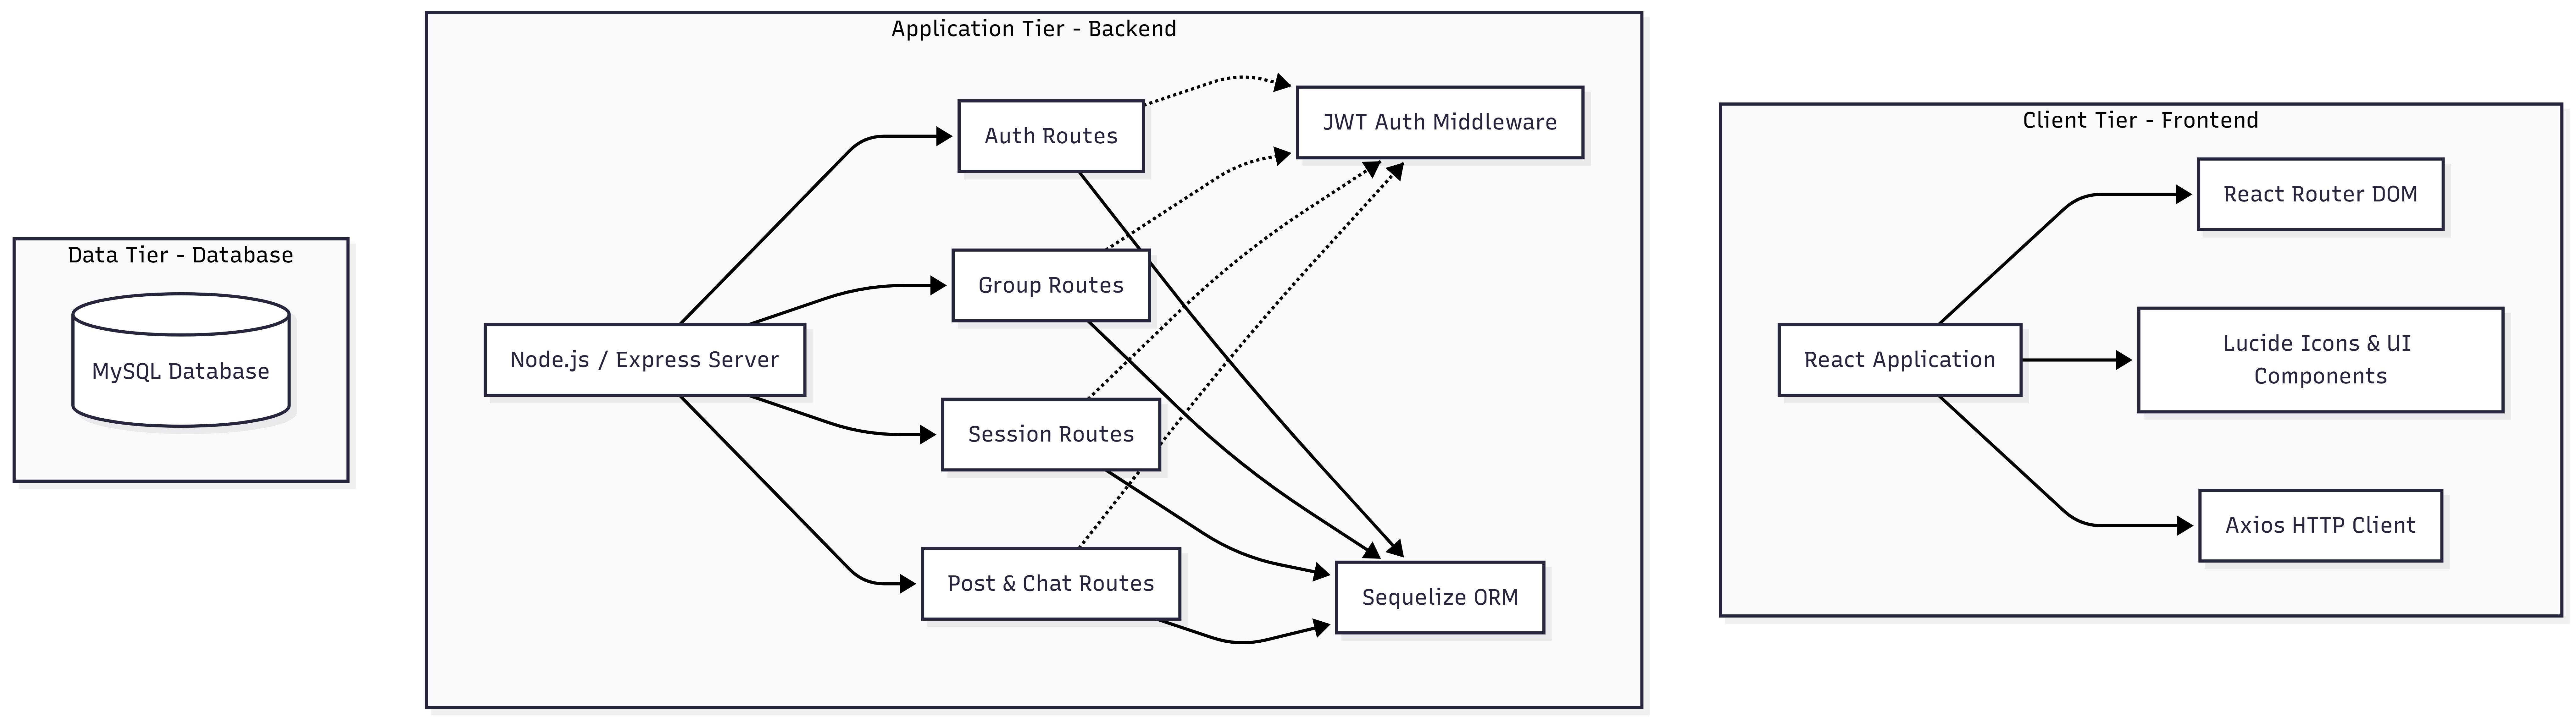
\includegraphics[width=\textwidth]{Client-Server-Architecture.png}
  \caption{System Architecture Diagram}
\end{figure}

\newpage

% -------------------------
% 4. DATABASE DESIGN
% -------------------------
\section{Database Design}
\subsection{ER Diagram}
The database design uses normalized relational modeling to reduce duplication and enforce referential integrity. Users can belong to multiple groups (many-to-many), and each group can contain multiple posts, sessions, and messages.

\begin{figure}[h!]
  \centering
  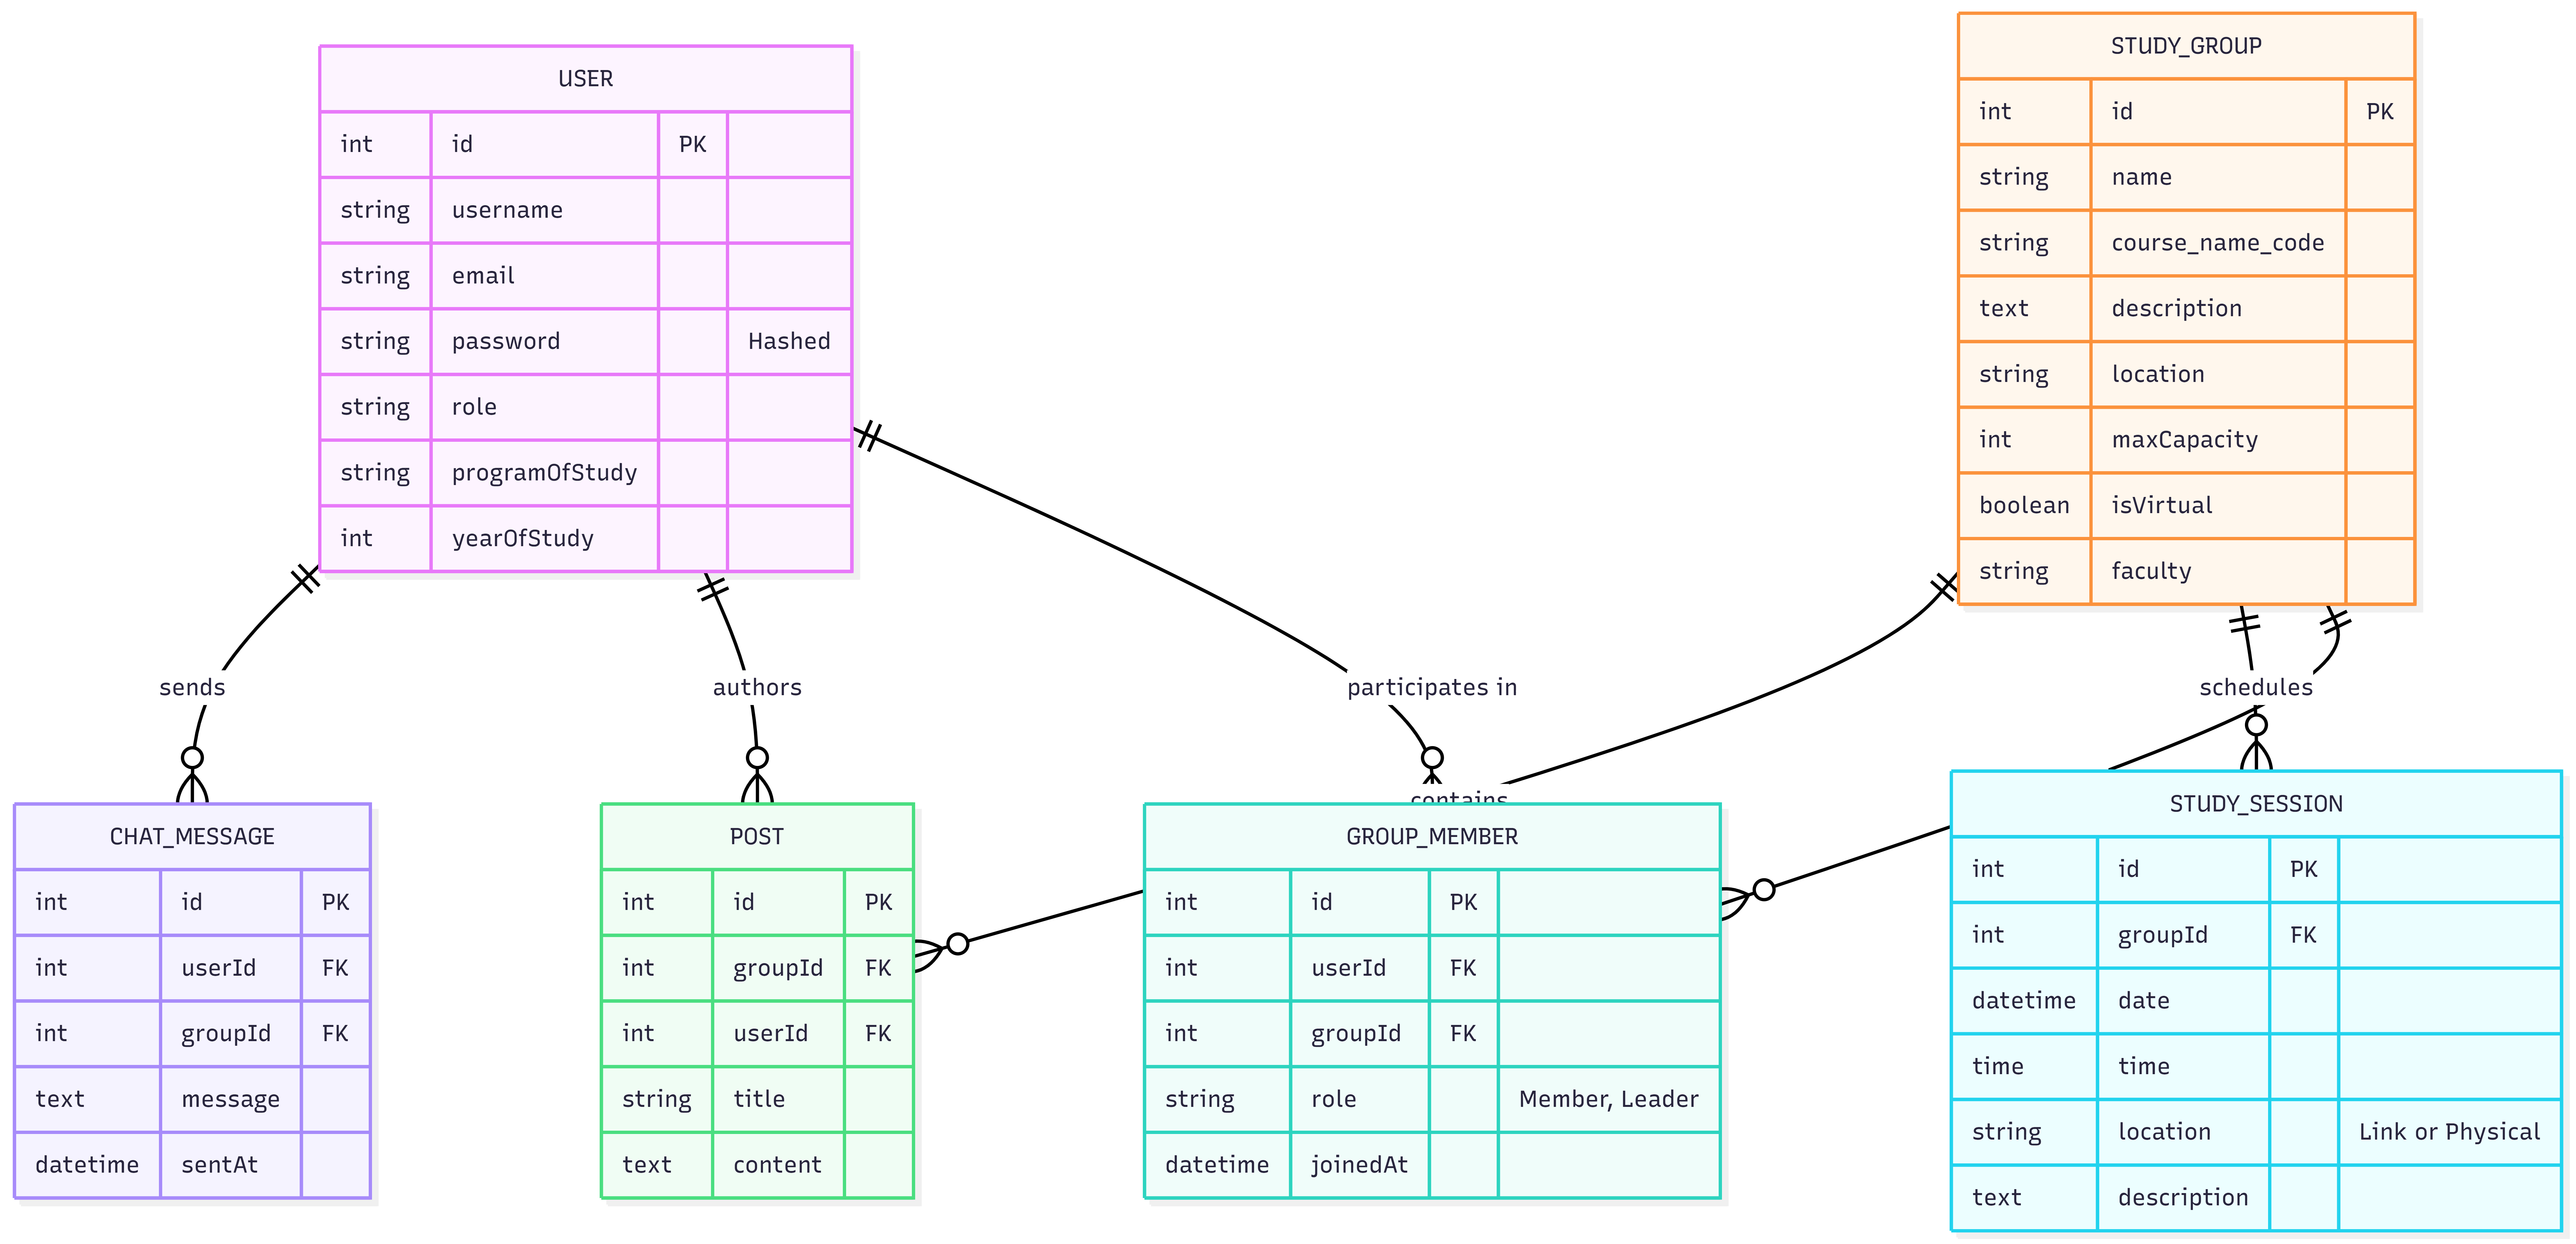
\includegraphics[width=\textwidth]{User-Engagement.png}
  \caption{Entity--Relationship Diagram}
\end{figure}

\subsection{Core Entities (Summary)}
\begin{itemize}
  \item \textbf{User}: Stores identity (name, email), role, and academic metadata (program and year).
  \item \textbf{Group}: Stores group details (course code/name, description, location, faculty, capacity, virtual flag).
  \item \textbf{GroupMember}: Junction table resolving many-to-many between users and groups, including group-level role (e.g., LEADER/member).
  \item \textbf{Session}: Stores scheduled study sessions per group (date, time, location/link, description).
  \item \textbf{Post}: Stores bulletin posts per group, authored by a user.
  \item \textbf{ChatMessage}: Stores chat messages per room with sender reference.
\end{itemize}

\newpage

% -------------------------
% 5. FUNCTIONAL REQUIREMENTS
% -------------------------
\section{Functional Requirements}
\subsection{Authentication}
\begin{itemize}
  \item Users can register with name, email, password, program of study, year of study, and role.
  \item Users can login and receive a JWT token.
  \item Authenticated users can retrieve their profile information.
\end{itemize}

\subsection{Study Groups}
\begin{itemize}
  \item Authenticated users can create groups and become group leaders.
  \item Users can browse and view group details.
  \item Users can join groups.
  \item Leaders can remove members (and users can remove themselves).
  \item Admins can assign group leaders and view join feedback (admin-only).
\end{itemize}

\subsection{Sessions and Communication}
\begin{itemize}
  \item Authenticated users can create and view group study sessions.
  \item Authenticated users can create and view posts within a group.
  \item Authenticated users can send and fetch chat messages (room-based).
\end{itemize}

% -------------------------
% 6. USER MANUAL
% -------------------------
\section{User Manual}
\subsection{Account Registration and Login}
\begin{itemize}
  \item Click \textbf{Register} and provide your full name, email, password, program of study, and year of study.
  \item After registration, click \textbf{Login} to authenticate and access your dashboard.
  \item The system uses JWT-based authentication for secured features.
\end{itemize}

\subsection{Discovering and Joining Study Groups}
\begin{itemize}
  \item Use the dashboard list and search/filter options to find groups by course, title, or faculty.
  \item Open a group to view details such as description, location, virtual/physical mode, and capacity.
  \item Click \textbf{Join Group} to become a member.
\end{itemize}

\subsection{Creating and Managing a Group (Leader)}
\begin{itemize}
  \item Select \textbf{Create Group} and enter group details (course, description, location, faculty, capacity).
  \item As creator, you become the \textbf{Group Leader} and can manage membership according to system rules.
\end{itemize}

\subsection{Scheduling Study Sessions}
\begin{itemize}
  \item Inside a group, select \textbf{Create Session} and provide date, time, location/link, and a short description.
  \item Members can view upcoming sessions from group pages or dashboard views.
\end{itemize}

\subsection{Posts and Chat}
\begin{itemize}
  \item Use group posts to share announcements, questions, and study material notes.
  \item Use chat for short real-time coordination; messages can be filtered by room.
\end{itemize}

\newpage

% -------------------------
% 7. API DOCUMENTATION
% -------------------------
\section{API Documentation}
\subsection{Base URL}
\begin{itemize}
  \item Local: \texttt{http://localhost:5000/api}
  \item Production: Replace with deployed API domain
\end{itemize}

\subsection{Authentication}
Protected endpoints require:
\begin{center}
\texttt{Authorization: Bearer <JWT\_TOKEN>}
\end{center}

\subsection{Endpoints Summary (Implemented)}
\noindent
\begin{tabularx}{\textwidth}{|>{\raggedright\arraybackslash}p{3.2cm}|X|}
\hline
\textbf{Endpoint} & \textbf{Purpose} \\ \hline
\texttt{GET /health} & API health check \\ \hline
\texttt{POST /auth/register} & Register a new user \\ \hline
\texttt{POST /auth/login} & Login and receive JWT \\ \hline
\texttt{GET /auth/me} & Get current user profile (protected) \\ \hline
\texttt{POST /groups} & Create a new group (protected) \\ \hline
\texttt{GET /groups} & List all groups \\ \hline
\texttt{GET /groups/:id} & Get group details \\ \hline
\texttt{POST /groups/:id/join} & Join a group (protected) \\ \hline
\texttt{DELETE /groups/:id/members/:userId} & Remove member (protected, rules apply) \\ \hline
\texttt{PUT /groups/:id/leader/:userId} & Assign leader (protected, admin only) \\ \hline
\texttt{GET /groups/feedback/admin/join} & Join feedback (protected, admin only) \\ \hline
\texttt{POST /sessions/group/:groupId} & Create group session (protected) \\ \hline
\texttt{GET /sessions/group/:groupId} & List group sessions (protected) \\ \hline
\texttt{POST /posts/group/:groupId} & Create group post (protected) \\ \hline
\texttt{GET /posts/group/:groupId} & List group posts (protected) \\ \hline
\texttt{POST /chat/messages} & Send chat message (protected) \\ \hline
\texttt{GET /chat/messages?room=...&limit=...} & Fetch messages (protected) \\ \hline
\end{tabularx}

\subsection{Common Error Responses}
\begin{itemize}
  \item \texttt{\{ "error": "Authentication token required" \}}
  \item \texttt{\{ "error": "Invalid or expired token" \}}
  \item \texttt{\{ "error": "Server error" \}}
\end{itemize}

\newpage

% -------------------------
% 8. INSTALLATION AND RUNNING
% -------------------------
\section{Installation and Running the System}
\subsection{Prerequisites}
\begin{itemize}
  \item Node.js (LTS recommended)
  \item MySQL Server
  \item Git
\end{itemize}

\subsection{Backend Setup (Express + MySQL)}
\begin{itemize}
  \item Navigate to the \texttt{backend} directory and install dependencies.
  \item Create \texttt{backend/.env} using \texttt{backend/.env.example} as a template.
  \item Required environment variables:
  \begin{itemize}
    \item \texttt{PORT} (default 5000)
    \item \texttt{DB\_HOST}, \texttt{DB\_USER}, \texttt{DB\_PASS}, \texttt{DB\_NAME}
    \item \texttt{JWT\_SECRET}
    \item \texttt{ADMIN\_SIGNUP\_CODE} (used for admin registration control)
  \end{itemize}
  \item Start the backend and verify \texttt{GET /api/health} returns a success response.
\end{itemize}

\subsection{Frontend Setup (React + Vite)}
\begin{itemize}
  \item Navigate to the \texttt{frontend} directory and install dependencies.
  \item Run the development server.
  \item For production deployments, configure \texttt{VITE\_API\_BASE\_URL} to point to the deployed backend API base URL.
\end{itemize}

% -------------------------
% 9. SECURITY CONSIDERATIONS
% -------------------------
\section{Security Considerations}
\begin{itemize}
  \item \textbf{JWT authentication}: Protected routes require a valid token.
  \item \textbf{Role-based access}: Certain operations (e.g., assigning leaders, admin feedback) require \texttt{ADMIN} role.
  \item \textbf{Database integrity}: Relational constraints and ORM validations help maintain consistent data.
  \item \textbf{CORS}: Local development is allowed by default; production should explicitly allow the deployed frontend origin(s).
\end{itemize}

% -------------------------
% 10. TESTING
% -------------------------
\section{Testing}
\begin{itemize}
  \item A Postman collection is provided for endpoint testing.
  \item A local test snapshot (2026-04-14) confirmed key endpoints including auth, groups, posts, sessions, and chat.
\end{itemize}

% -------------------------
% 11. DEPLOYMENT (SUMMARY)
% -------------------------
\section{Deployment Summary}
The recommended deployment order is:
\begin{itemize}
  \item Deploy backend first to a Node-compatible host and set environment variables.
  \item Update backend CORS to allow the Netlify domain(s).
  \item Deploy the frontend to Netlify and set \texttt{VITE\_API\_BASE\_URL}.
  \item Add SPA routing fallback for React Router deep links.
\end{itemize}

% -------------------------
% 12. CONCLUSION
% -------------------------
\section{Conclusion}
The Student Study Group Finder provides a secure and practical platform for students to collaborate through study groups, scheduled sessions, and structured communication. The chosen architecture and technology stack support modular development, secure access control, and scalable data management suitable for campus-wide use.

% -------------------------
% APPENDIX
% -------------------------
\appendix
\section{Appendix: Environment Variables (Backend)}
\noindent
Template from \texttt{backend/.env.example}:
\begin{itemize}
  \item \texttt{PORT=5000}
  \item \texttt{DB\_HOST=localhost}
  \item \texttt{DB\_USER=your\_mysql\_user}
  \item \texttt{DB\_PASS=your\_mysql\_password}
  \item \texttt{DB\_NAME=study\_group\_finder}
  \item \texttt{JWT\_SECRET=replace\_with\_strong\_jwt\_secret}
  \item \texttt{ADMIN\_SIGNUP\_CODE=replace\_with\_admin\_signup\_code}
\end{itemize}

\end{document}
